\setcounter{section}{6}
\phantomsection
\section*{Results}
\addcontentsline{toc}{section}{Results}

This section provides the empirical findings on birth order and scholarly productivity.
We start by outlining the brother pair sample and key productivity trends.
We then compare older and younger brothers through paired differences, before moving to regression-based estimates that control for family characteristics, age gaps, and institutional context.
Finally, we investigate whether differences in inheritance systems are associated with differences in birth-order productivity patterns and provide multiple robustness checks.

\phantomsection
\subsection*{4.1 Descriptive statistics}
\addcontentsline{toc}{subsection}{4.1 Descriptive statistics}

Summary statistics for the sample of rankable brother pairs are provided in Table \ref{tab:descriptives}. There are 619 pairs of brothers in this dataset, for whom we can determine birth order. For siblings, the average age gap is 7.2 years. About 40\% of the scholars in our sample had a father who also worked in academia.

Older brothers seem to be slightly more productive on average when it comes to scholarly production. The average number of titles associated with VIAF is 12.3 (older brothers) and 10.0 (younger brothers). But this difference in averages does not mean that older brothers always outshine their younger siblings. Figure \ref{fig:birthorder_pie} illustrates the distribution of within-family productivity comparisons: older brothers are more productive in 42\% of pairs, while younger brothers outperform their older siblings in about 32\% of cases, and productivity is equal in the remaining pairs. This statistic reflects the frequency with which one sibling outperforms the other, not the magnitude of productivity differences. This implies significant heterogeneity in within-family productivity differences. This family-specific pattern is consistent with the highly skewed distribution of scholarly output: for some families, the older brother is much more productive and, for many other families, productivity levels are fairly similar. Overall, the evidence points to a modest average productivity advantage for older brothers rather than a universal birth-order effect.

\begin{figure}[htbp]
\centering
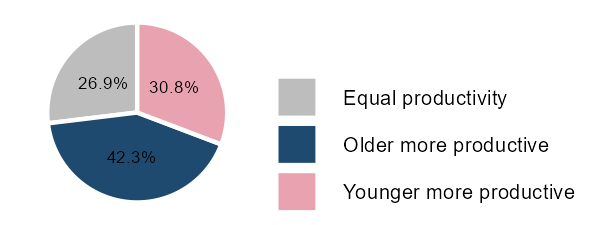
\includegraphics[width=0.65\textwidth]{figures/Pie_Productivity_BirthOrder.png}
\caption{Productivity comparison between older and younger brothers}
\label{fig:birthorder_pie}
\begin{minipage}{0.85\textwidth}
\footnotesize
\textit{Notes:} The figure shows the distribution of within-family productivity comparisons between older and younger brothers. Shares indicate the proportion of brother pairs in which the older brother has more titles recorded in VIAF, the younger brother has more titles, or both brothers have the same number of titles. 
\end{minipage}
\end{figure}
\FloatBarrier

\begin{table}[H]
\centering
\caption{Descriptive Statistics}
\label{tab:descriptives}

\begin{tablebody}
\begin{tabular}{l c}
\toprule
\textbf{Statistic} & \textbf{Value} \\
\midrule
Number of brother pairs & 645 \\
Mean entry age in academia & 32.93 \\
Mean age gap (years) & 7.22 \\
Father in academia (share) & 38.8\% \\
Titles (older brother) & 11.89 \\
Titles (younger brother) & 9.79 \\
Older brother more productive (share) & 41.6\% \\
Younger brother more productive (share) & 31.3\% \\
Share of individuals with no titles & 40.2\% \\
Share of pairs with no titles & 25.4\% \\
\bottomrule
\end{tabular}
\end{tablebody}

\vspace{4pt}
\begin{minipage}{\textwidth}
\footnotesize
\textit{Notes:} Descriptive statistics for the sample of rankable brother pairs, i.e. pairs for which birth order can be identified, unless otherwise indicated. Scholarly productivity is measured using the number of titles recorded in VIAF. The mean entry age into academia is computed using all scholars with available information on birth year and first recorded academic activity. Shares are reported as percentages.
\end{minipage}

\end{table}
\FloatBarrier

The inverse hyperbolic sine transformed input of titles provides the older and younger brothers scholarly productivity distribution as shown on Figure \ref{fig:titles_distribution}. The two distributions mostly overlap, suggesting that the differences in productivity between families is small on average. But the distribution of older brothers is shifted a little to the right, indicating a slight bump in scholarly output. The concentration of observations along the zero axis is high because most scholars in the dataset have few titles recorded, a fact consistent with historical productivity distributions being skewed.

\begin{figure}[H]
\centering
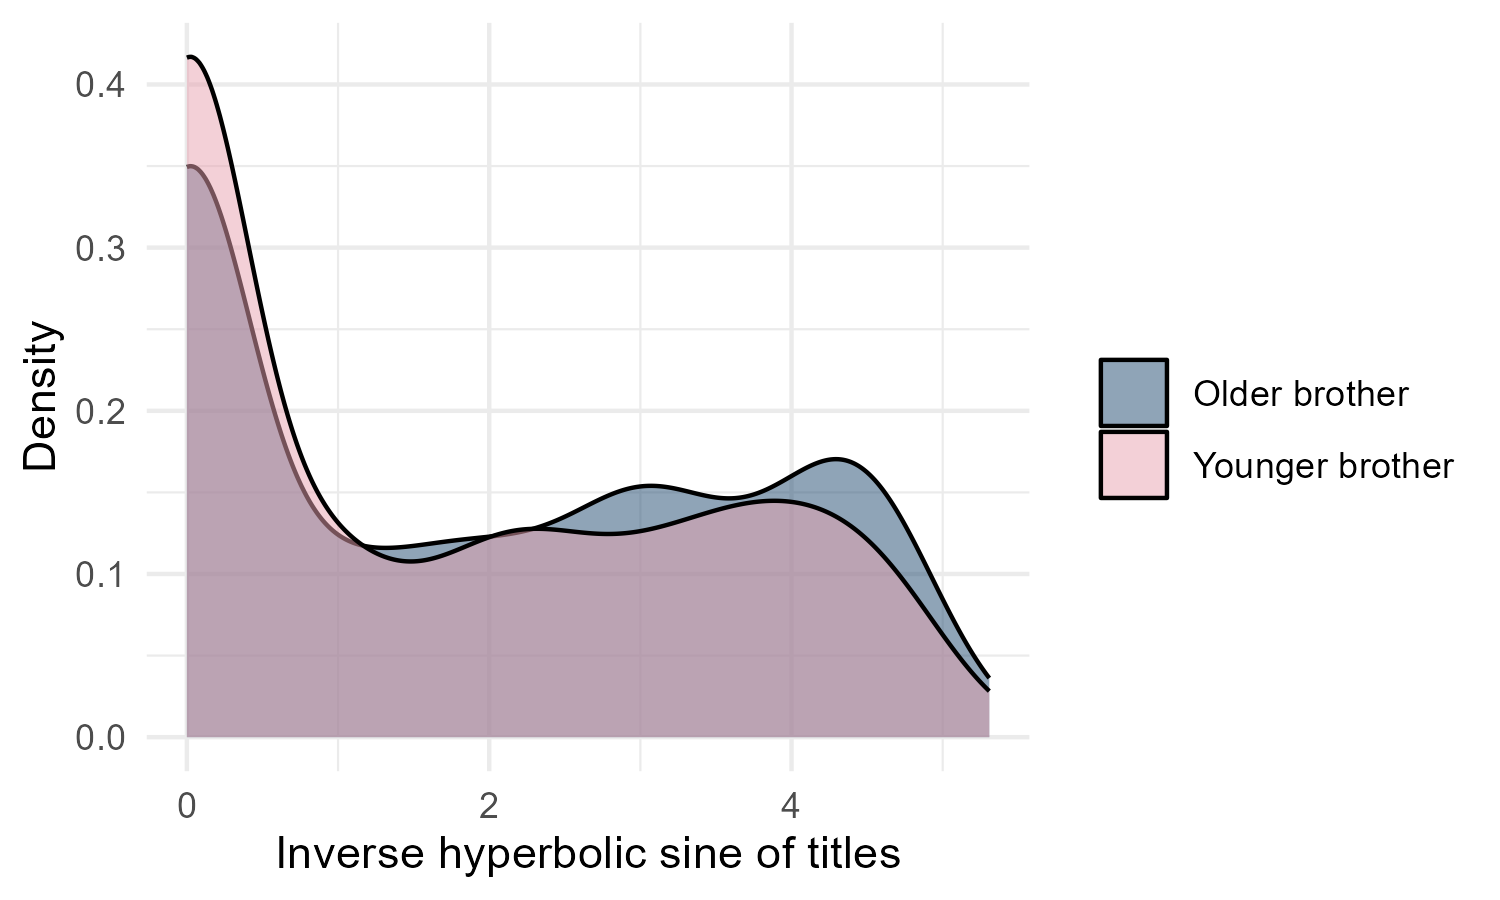
\includegraphics[width=0.8\textwidth]{figures/Plot_Productivity_Distribution.png}
\caption{Distribution of scholarly productivity by birth order}
\label{fig:titles_distribution}
\begin{minipage}{0.85\textwidth}
\footnotesize
\textit{Notes:} The figure compares the distribution of scholarly productivity between older and younger brothers. Productivity is measured using the inverse hyperbolic sine transformation of the number of titles recorded in VIAF. The transformation allows the inclusion of zero values and reduces the influence of extreme observations.
\end{minipage}
\end{figure}
\FloatBarrier

\phantomsection
\subsection*{4.2 Paired comparisons between brothers}
\addcontentsline{toc}{subsection}{4.2 Paired comparisons between brothers}

In order to provide a first assessment of the differences in productivity by birth-order, Table \ref{tab:ttests} displays paired comparisons of older and younger brothers over multiple measures of scholarly productivity and visibility.

Older brothers tend to perform slightly better than their younger siblings on several measures of scholarly productivity on average. For instance, older brothers hold on average 2.35 more titles in VIAF than their younger siblings; this difference is statistically significant at conventional levels. Using the inverse hyperbolic sine transformation of titles, this estimated gap is equivalent to approximately a 30\% higher level of productivity in older brothers.

The same patterns emerge when we look at other measures of scholarly prominence. Older siblings have longer Wikipedia pages, more versions in other languages on Wikipedia, more publishers, and more coauthors with their publications. They are also more likely to have at least one title recorded in VIAF.

These findings align with a slight advantage for firstborn children in academic visibility and productivity. However, the size of these differences varies by indicator and are not statistically significant for all outcomes.

\begin{table}[H]
\centering
\caption{Paired Differences Between Older and Younger Brothers}
\label{tab:ttests}

\begin{tablebody}
\begin{tabular}{l c c c c}
\toprule
\textbf{Measure} & \textbf{Mean Diff.} & \textbf{p-value} & \textbf{N} \\
\midrule
Titles (VIAF) & 2.096 & 0.0076 & 645 \\
Titles (VIAF, asinh) & 0.245 & 0.0007 & 645 \\
Longest Wikipedia page (chars) & 409.788 & 0.0453 & 645 \\
Longest Wikipedia page (asinh) & 0.182 & 0.0228 & 645 \\
Has at least one title & 0.056  & 0.0089 & 645 \\
Number of Wikipedia languages & 0.659 &  0.0215 & 645 \\
Publication countries (VIAF) & 0.372 &  0.0140 & 645 \\
Publishers (VIAF) & 0.667 & 0.0043 & 645 \\
Coauthors (VIAF) & 1.056 & 0.0001 & 645 \\
Publications with ISBN & 0.381 & 0.1158 & 645 \\
Publications before 1900 & 21.667  & 0.0013 & 645 \\
Publications after 1900 & 1.932  & 0.1904 & 645 \\
Academic affiliations (Wikidata) & 0.130  & 0.0626 & 645 \\
Number of occupations (Wikidata) & 0.171  & 0.0328 & 645 \\
Number of positions & -0.033  & 0.5849 & 645 \\
Longevity (years) & -0.180  & 0.8297 & 579 \\
\bottomrule
\end{tabular}
\end{tablebody}

\vspace{4pt}
\begin{minipage}{\textwidth}
\footnotesize
\textit{Notes:} Paired t-tests comparing older and younger brothers across productivity and recognition measures. Mean differences are calculated as older minus younger. Variables transformed using the inverse hyperbolic sine transformation are discussed in the main text.
\end{minipage}

\end{table}
\FloatBarrier

\phantomsection
\subsection*{4.3 Extensive and intensive margins of productivity}
\addcontentsline{toc}{subsection}{4.3 Extensive and intensive margins of productivity}

In order to better understand the drivers of the productivity differences, we decompose scholarly production into extensive and intensive margins. This distinction enables us to determine whether birth order predicts the chances of becoming a productive scholar or the productivity level among those who do publish.

The extensive margin is the probability that a scholar has at least one title linked to her name. The intensive margin is the number of titles conditional on having published at least one title.

Table \ref{tab:extensive_intensive} shows regression estimates for these two margins. More precisely, the extensive-margin specification is based on a logit model whereas for the intensive-margin specification it is OLS regression with inverse hyperbolic sine transformation of titles.

The key finding is that older brothers are more likely to have one or more publications recorded. The coefficient on the indicator that the sibling is an older brother is positive and statistically significant, thus indicating a birth order effect in terms of increasing the probability to enter scholarly production.

In comparison, conditional on publishing at least one work the productivity advantage of older brothers is smaller and only marginally significant. This would imply that birth order matters more for entry to scholarly activity than for conditional productivity.

\begin{table}[H]
\centering
\caption{Extensive and Intensive Margins of Scholarly Productivity}
\label{tab:extensive_intensive}

\begin{tablebody}
\begin{tabular}{l c c}
\toprule
 & \textbf{Extensive (Logit)} & \textbf{Intensive (OLS)} \\
 & \textit{Pr(Title $>0$)} & \textit{Asinh titles} \\
\midrule

Constant
& 0.051 & 2.892*** \\
& (0.129) & (0.101) \\

Older sibling
& 0.238*** & 0.141 \\
& (0.091) & (0.089) \\

Age gap
& -0.002 & -0.013 \\
& (0.012) & (0.009) \\

Father in academia
& 0.654*** & 0.090 \\
& (0.176) & (0.112) \\

\midrule
Clustered SE (family) & Yes & Yes \\
\midrule
Observations & 1290 & 772 \\
R$^{2}$ &  & 0.008 \\
Adj. R$^{2}$ &  & 0.004 \\
\bottomrule
\end{tabular}
\end{tablebody}

\vspace{4pt}
\begin{minipage}{\textwidth}
\footnotesize
\textit{Notes:} Column (1) reports logit estimates for the probability of having at least one title recorded in VIAF. Column (2) reports OLS estimates conditional on positive titles using the inverse hyperbolic sine transformation of titles. Standard errors are clustered at the family level. \textit{Significance levels:} *** $p<0.01$, ** $p<0.05$, * $p<0.10$.
\end{minipage}

\end{table}
\FloatBarrier

\phantomsection
\subsection*{4.4 Inheritance systems}
\addcontentsline{toc}{subsection}{4.4 Inheritance systems}

Before looking at the role of inheritance systems in a regression analysis, we first present their geographical and historical distribution, respectively, in the sample.

The regimes of inheritance are assigned to scholars' places of birth using Todd's classification on European family systems. Each birthplace is linked to a NUTS3 region and fully inherits the institutional regime of that area.

At the same time, Figure \ref{fig:todd_map} shows where these inheritance systems are located and where scholars from dataset were born. Shaded areas represent Todd’s typology of inheritance systems, and the circles show where scholars in the sample were born. The size of the circles corresponds to how many scholars are related to each birthplace.

\begin{figure}[htbp]
\centering
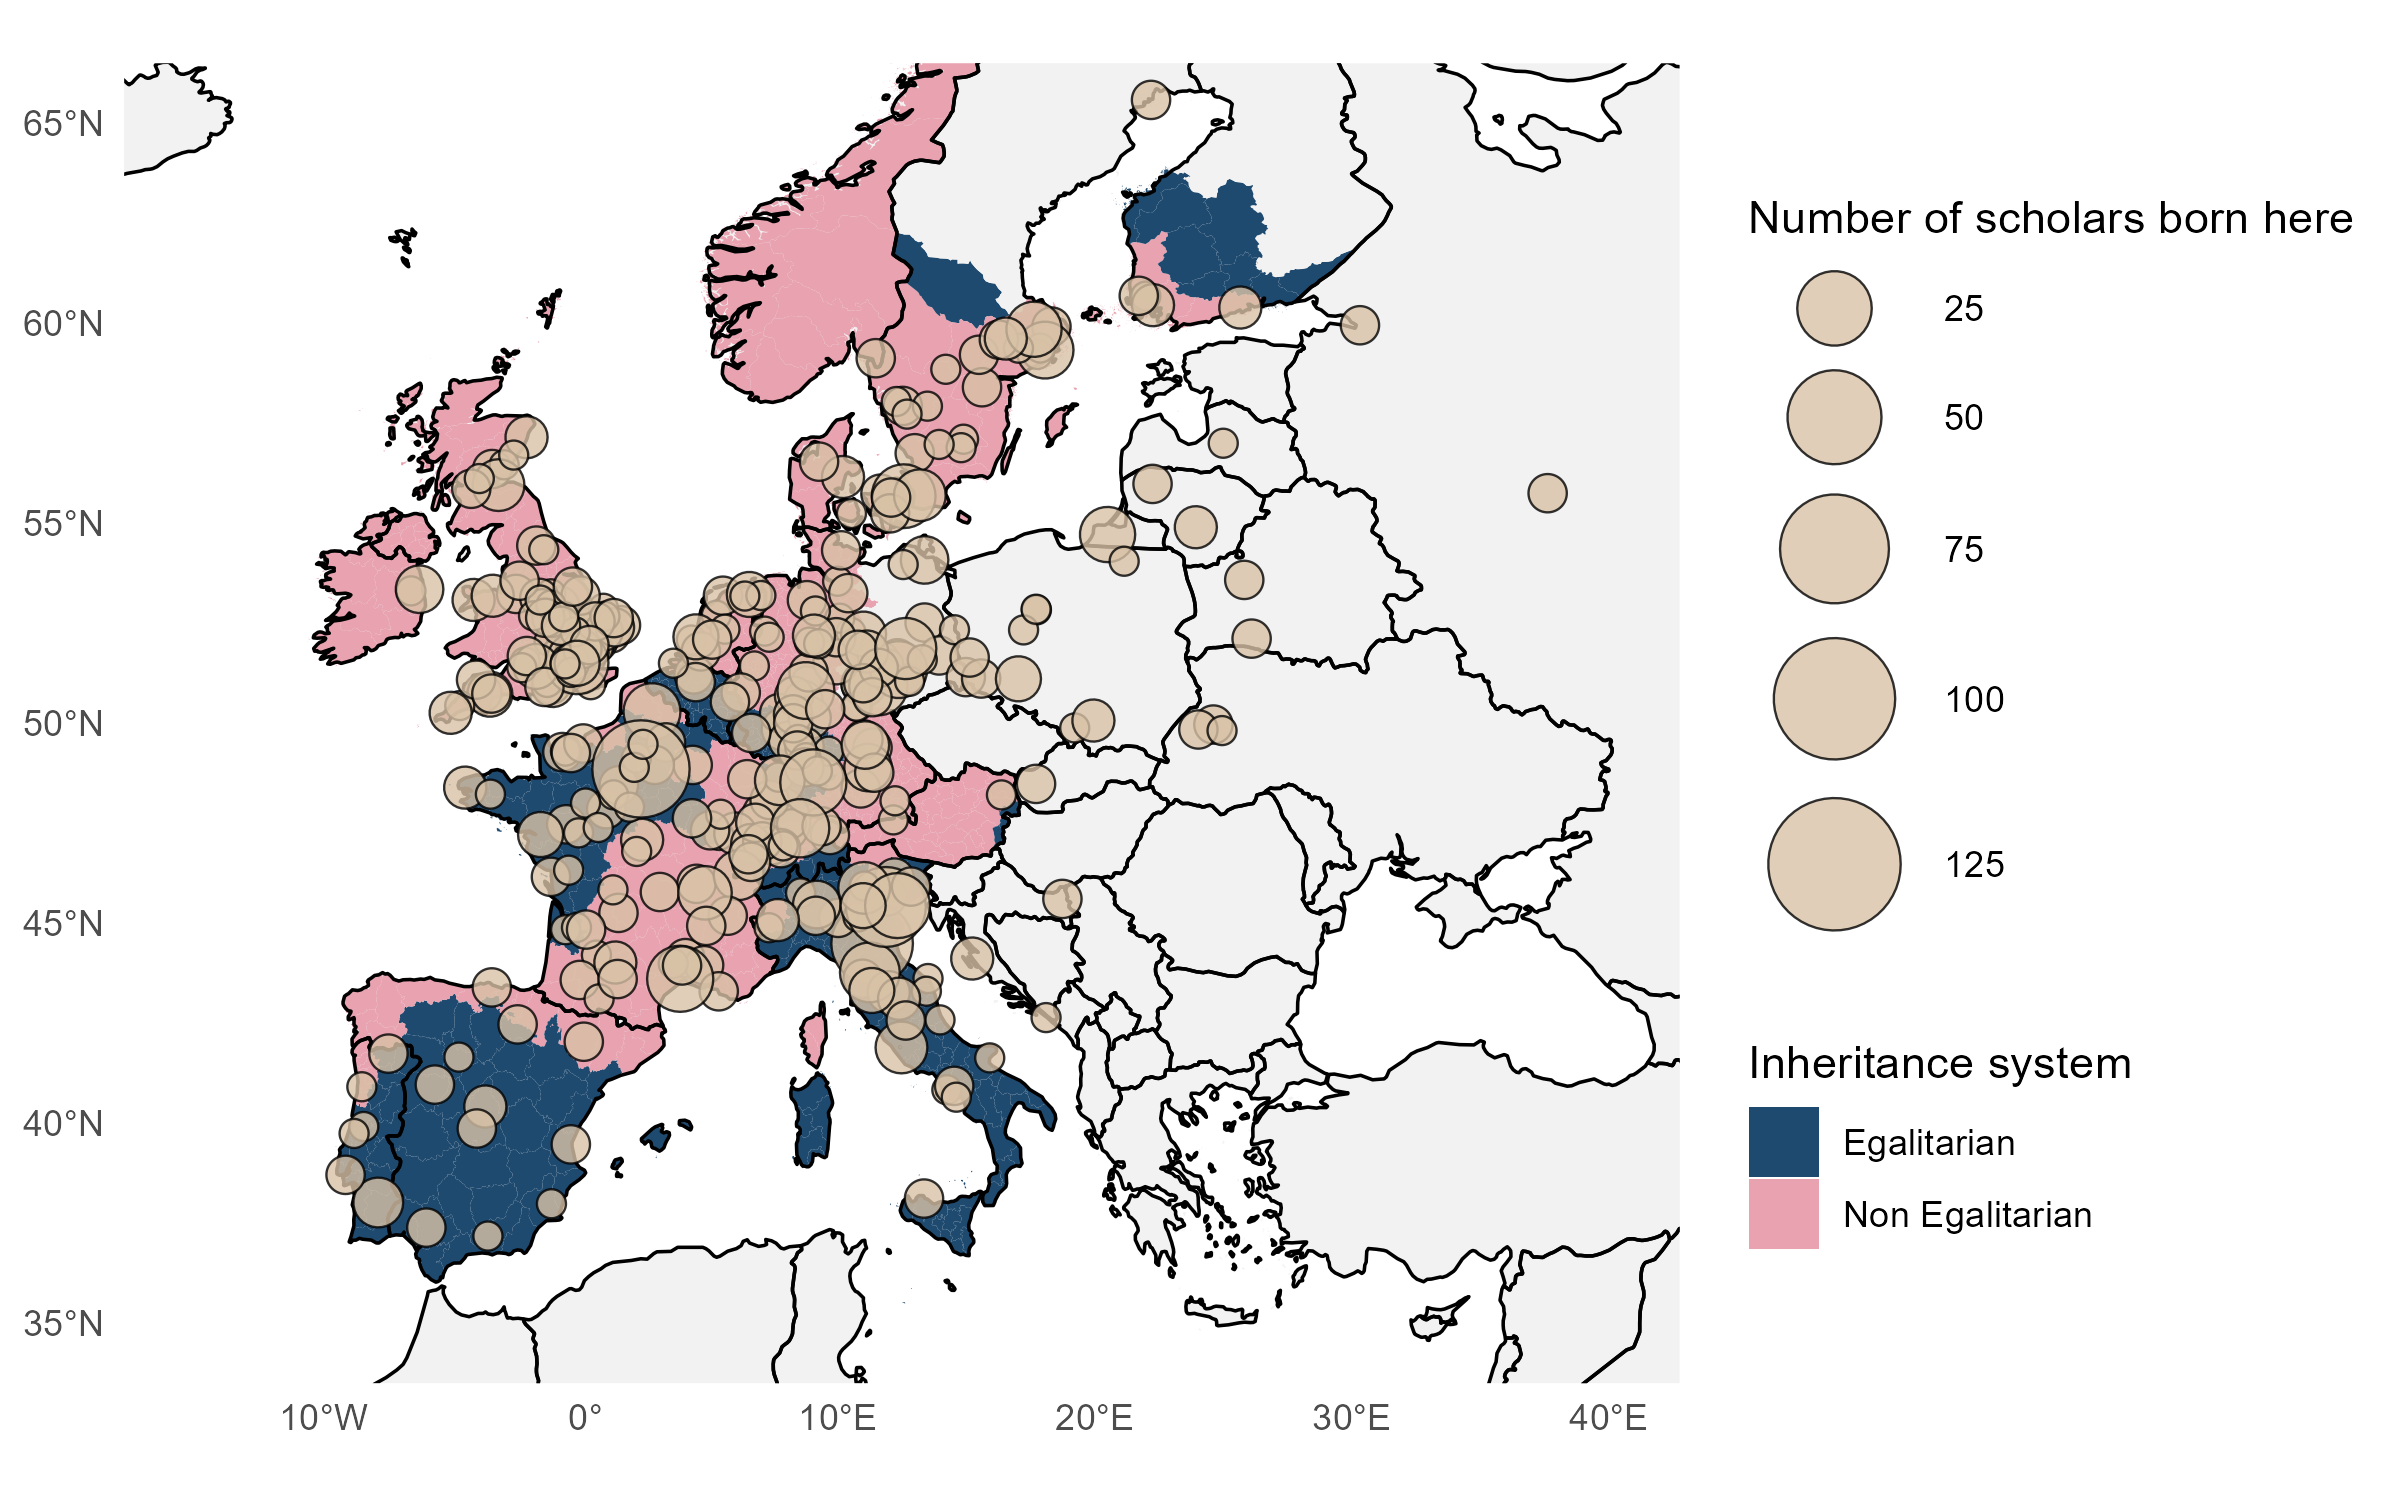
\includegraphics[width=\textwidth]{figures/Map_Birthplaces_ToddColors.png}
\caption{Birthplaces of Scholars and Inheritance Systems in Europe}
\label{fig:todd_map}

\begin{minipage}{0.85\textwidth}
\footnotesize
\textit{Notes:} The map displays the birthplaces of scholars in the dataset and the classification of inheritance systems across European regions. Inheritance regimes are assigned at the NUTS3 level following Todd's classification. Circles indicate the number of scholars born in each location.
\end{minipage}

\end{figure}
\FloatBarrier

In fact scholars from the dataset can be found throughout much of Europe in a diverse array of historical regions with differing inheritance institutions (Figure \ref{fig:todd_map}). This variation in space is our foundation to explore whether different family inheritance structures correlate with sibling differences in scholarly productivity.

Table \ref{tab:inheritance} shows the sample composition classified according to Todd's typology. About 61\% of the observations correspond to regions with non-egalitarian inheritance systems and the remaining 39\% correspond to egalitarian ones.

In order to get a better sense of the time dimension of this variation, we plot in Figure \ref{fig:inheritance_century} the proportion of brother pairs born in regions that exhibit non-egalitarian inheritance systems at each century.

\begin{figure}[htbp]
\centering
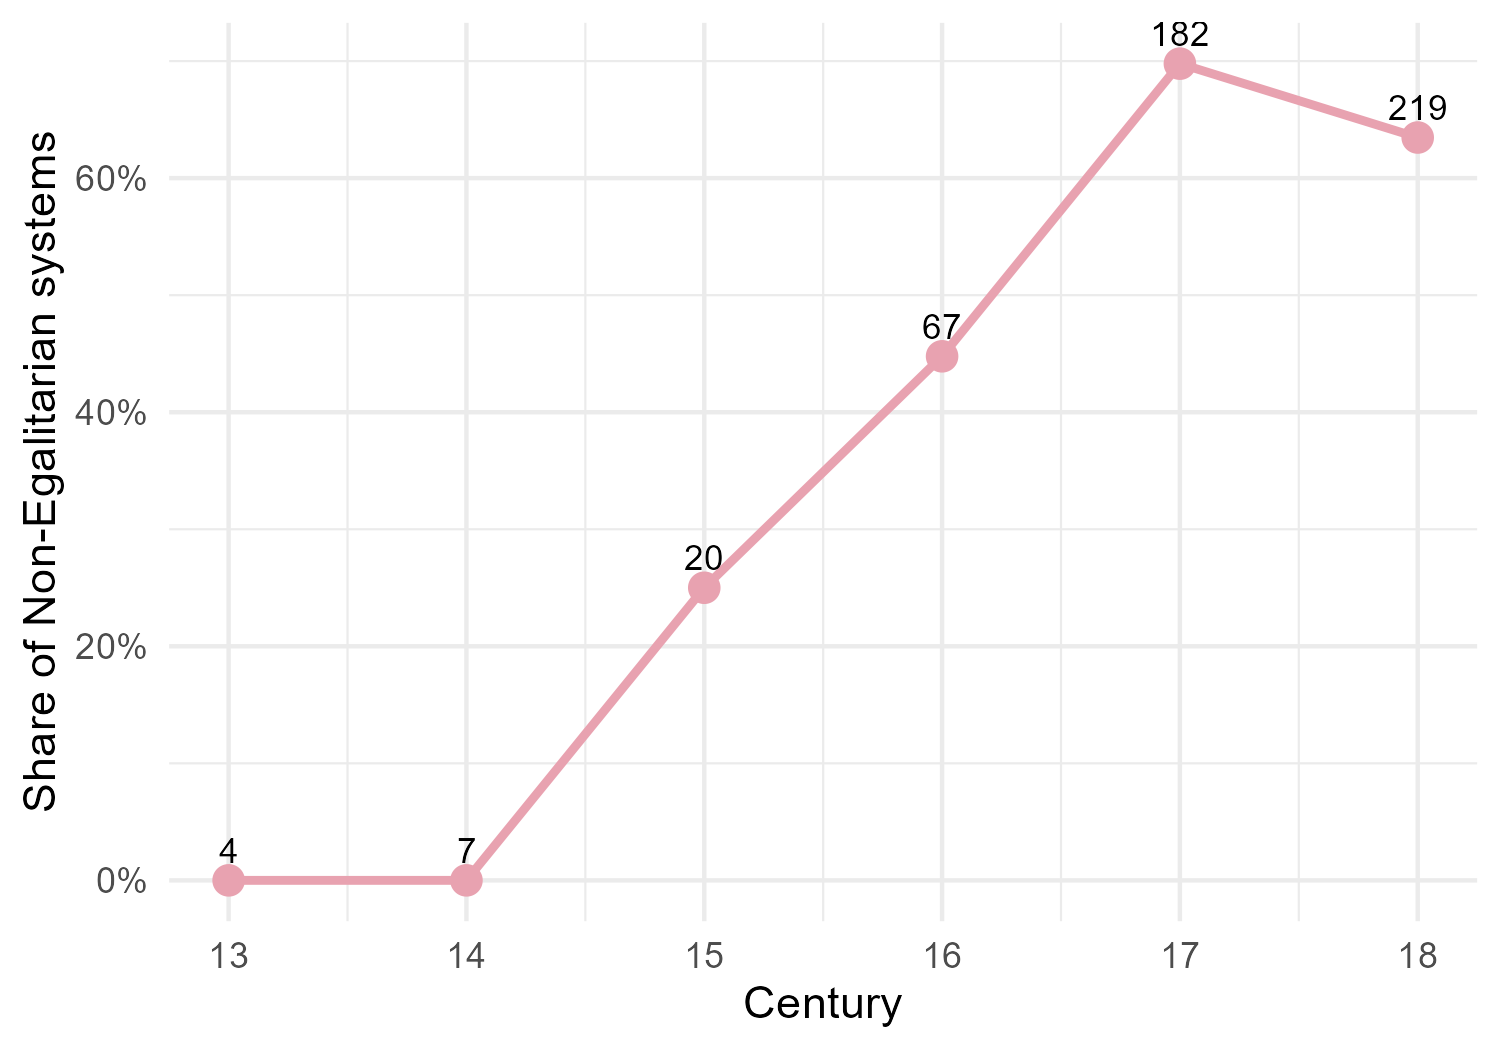
\includegraphics[width=0.8\textwidth]{figures/Inheritance_by_Century.png}
\caption{Share of Non-Egalitarian Inheritance Systems by Century}
\label{fig:inheritance_century}

\begin{minipage}{0.85\textwidth}
\footnotesize
\textit{Notes:} The figure shows the share of brother pairs born in regions with non-egalitarian inheritance systems by century. Shares are computed among observations with classified inheritance systems (egalitarian or non-egalitarian). The numbers above each point indicate the total number of observations in that century. Inheritance systems are assigned at the NUTS3 level following Todd's classification.
\end{minipage}

\end{figure}
\FloatBarrier

Figure \ref{fig:inheritance_century} suggests that non-egalitarian inheritance systems are still widespread across the sample, although with differences of relative importance in different historical periods. The variation, both across space and over time, provides the empirical foundation for testing whether differences in inheritance institutions influence disparities in scholarly productivity of older and younger brothers.

\phantomsection
\subsection*{4.5 Regression analysis}
\addcontentsline{toc}{subsection}{4.5 Regression analysis}

Next, we estimate regression models that investigate the determinants of the birth-order productivity gap while controlling for observable characteristics.

The response variable is the inverse hyperbolic sine transformation of the difference in title count registered at VIAF between older and younger brothers. Thus, positive values signal greater scholarly productivity for the older sibling. Various metrics of scholarly visibility were discussed in the paired comparisons, but in the regression, titles are used as the main measure of academic output. While other variables in the dataset, such as Wikipedia page length, number of languages, or publishers, capture more general aspects of this visibility and diffusion than its production, titles are the most direct and consistent observable measure available to act as a proxy for scholarly output. Titles, furthermore, are uniformly entered in the historical sources used in the dataset, making them far more comparable across scholars and centuries than other indicators of visibility.

Table \ref{tab:main_regressions} reports the results. Column (1) shows the specification with only the age gap between brothers. Column (2) adds family background and institutional overlap controls. Column (3) co-adds the inheritance system, distinguishing between egalitarian and non-egalitarian inheritance regimes. Lastly, Column (4) also adds century fixed effects to control for wider historical shifts in academic institutions and scholarly production.

In all specifications, larger age gaps between siblings lead to a larger productivity advantage for the older brother. In quantitative terms, the estimates suggest that a one-year increase in the age gap yields about 2–3\% more of a productivity advantage for the older sibling, which translates to approximately 20–30\% difference given an age gap of ten years.

Family background also seems to count. For pairs in which the father was active in academia, productivity was more equal between siblings, a sign that they likely had the same access to academic networks or resources. We find that brothers who overlap within the same academic institution exhibit smaller productivity gaps.

In systems with inheritance, the coefficient for non-egalitarian inheritance is positive but not statistically precise. In order to further examine whether or not the relationship between inheritance institutions and the birth-order productivity gap differs across historical periods, Appendix Table~\ref{tab:inheritance_century} presents specifications which respectively interact inheritance systems with an indicator for the century. While several interaction coefficients are statistically positive, such estimates are imprecise and should therefore not be over-interpreted.

Overall, the regression results suggest a modest but robust birth-order advantage in scholarly productivity among families.

\begin{table}[H]
\centering
\caption{Determinants of the Birth-Order Productivity Gap}
\label{tab:main_regressions}

\begin{tablebody}
\begin{tabular}{l c c c c}
\toprule
 & (1) & (2) & (3) & (4)\\
 & \multicolumn{4}{c}{\textit{Asinh difference in titles}} \\
\midrule

Constant
& 0.083
& 0.023
& 0.005
& -0.162 \\
& (0.109)
& (0.126)
& (0.177)
& (0.197) \\

Age gap 
& 0.023** & 0.022** & 0.022** & 0.019* \\
& (0.010) & (0.010) & (0.010) & (0.011) \\

Father in academia 
&  & -0.184 & -0.186 & -0.163 \\
&  & (0.149) & (0.148) & (0.150) \\

Different institution 
&  & 0.440** & 0.440** & 0.485*** \\
&  & (0.181) & (0.181) & (0.180) \\

Non-egalitarian inheritance 
&  &  & 0.031 & 0.135 \\
&  &  & (0.169) & (0.175) \\

Unknown inheritance system
&  &  & 0.019 & 0.130 \\
&  &  & (0.198) & (0.205) \\

13th century
& & & & 0.099 \\
& & & & (0.223) \\

14th century
& & & & 1.764*** \\
& & & & (0.552) \\

15th century
& & & & 0.863** \\
& & & & (0.345) \\

16th century
& & & & 0.025 \\
& & & & (0.226) \\

17th century
& & & & 0.099 \\
& & & & (0.161) \\

\midrule
Century controls & No & No & No & Yes \\
Clustered SE (family) & Yes & Yes & Yes & Yes \\
\midrule
Observations & 645 & 645 & 645 & 645 \\
R$^{2}$ & 0.005 & 0.020 & 0.020 & 0.035 \\
Adj. R$^{2}$ & 0.004 & 0.015 & 0.012 & 0.020 \\
\bottomrule
\end{tabular}
\end{tablebody}

\vspace{4pt}
\begin{minipage}{\textwidth}
\footnotesize
\textit{Notes:} The dependent variable is the inverse hyperbolic sine (asinh) difference in titles between older and younger brothers. Positive values indicate higher productivity for the older sibling. Standard errors clustered at the family level are reported in parentheses. Column (4) includes century indicator variables, with the 18th century used as the omitted reference category.

\textit{Significance levels:} *** $p<0.01$, ** $p<0.05$, * $p<0.10$.
\end{minipage}

\end{table}
\FloatBarrier

\phantomsection
\subsection*{4.6 Robustness checks}
\addcontentsline{toc}{subsection}{4.6 Robustness checks}

Several different specifications and sample restrictions are applied in order to test robustness of the birth-order results.

Firstly, we limit the sample to brother pairs with an age difference of no more than twenty years (Table~\ref{tab:robustness}, Column 1). This addresses the concern that very large age differences between siblings may have more to do with differences in generational context than actual sibling comparisons. The estimated coefficients continue very similar in terms of magnitude to the baseline results, implying that the primary findings usually are not driven by excessive age variations.

Secondly, we limit the sample to families with two sons (Table~\ref{tab:robustness}, Column 2). This specification removes cases in which larger families generate multiple brother pairs and therefore focuses on simpler sibling structures. As the sample size shrinks, the estimated coefficients are still fairly close to those shown in baseline specification.

Thirdly, we repeat the analysis with alternative measures of scholarly visibility (table~\ref{tab:alt_measures}). Furthermore, we look at the length of the scholar's Wikipedia page, the number of language versions that exist on Wikipedia, and the number of publishers associated with their works. These variables represent more general aspects of scholarly visibility. Estimates obtained with these alternative measures are somewhat less precise in general, mirroring the noisier nature of these particular indicators of scholarly prominence.

The robustness exercises considered together suggest that the main findings are not coming from specific sample choices or from the particular measure of scholarly productivity employed. Though the magnitude of the coefficients differs between specifications, the overall pattern is consistently aligned with a modest birth-order effect in scholarly output.